\documentclass{article}
\usepackage[a4paper, margin=1in]{geometry} % Adjust margin size as needed
\usepackage{graphicx} % Required for inserting images
\usepackage{listings}
\lstset{basicstyle=\ttfamily}
\usepackage{float}
\usepackage{courier}
\usepackage{tabularx}
\usepackage{tikz}
\usepackage{url}
\usepackage{amsmath}
\usepackage{float}
\usepackage{hyperref}
\usepackage{MnSymbol}
\usepackage{indentfirst}

\title{Project \#1 - Indexer/Search Engine}
\author{Daniel Marin and Jennifer Vicentes}
\date{October , 2024}

\begin{document}
\maketitle
\tableofcontents
\section{Class Diagram}
The Class Diagram contained several changes throughout the development of the code. The original Class Diagram we developed was:
\begin{figure}[H]
    \centering
    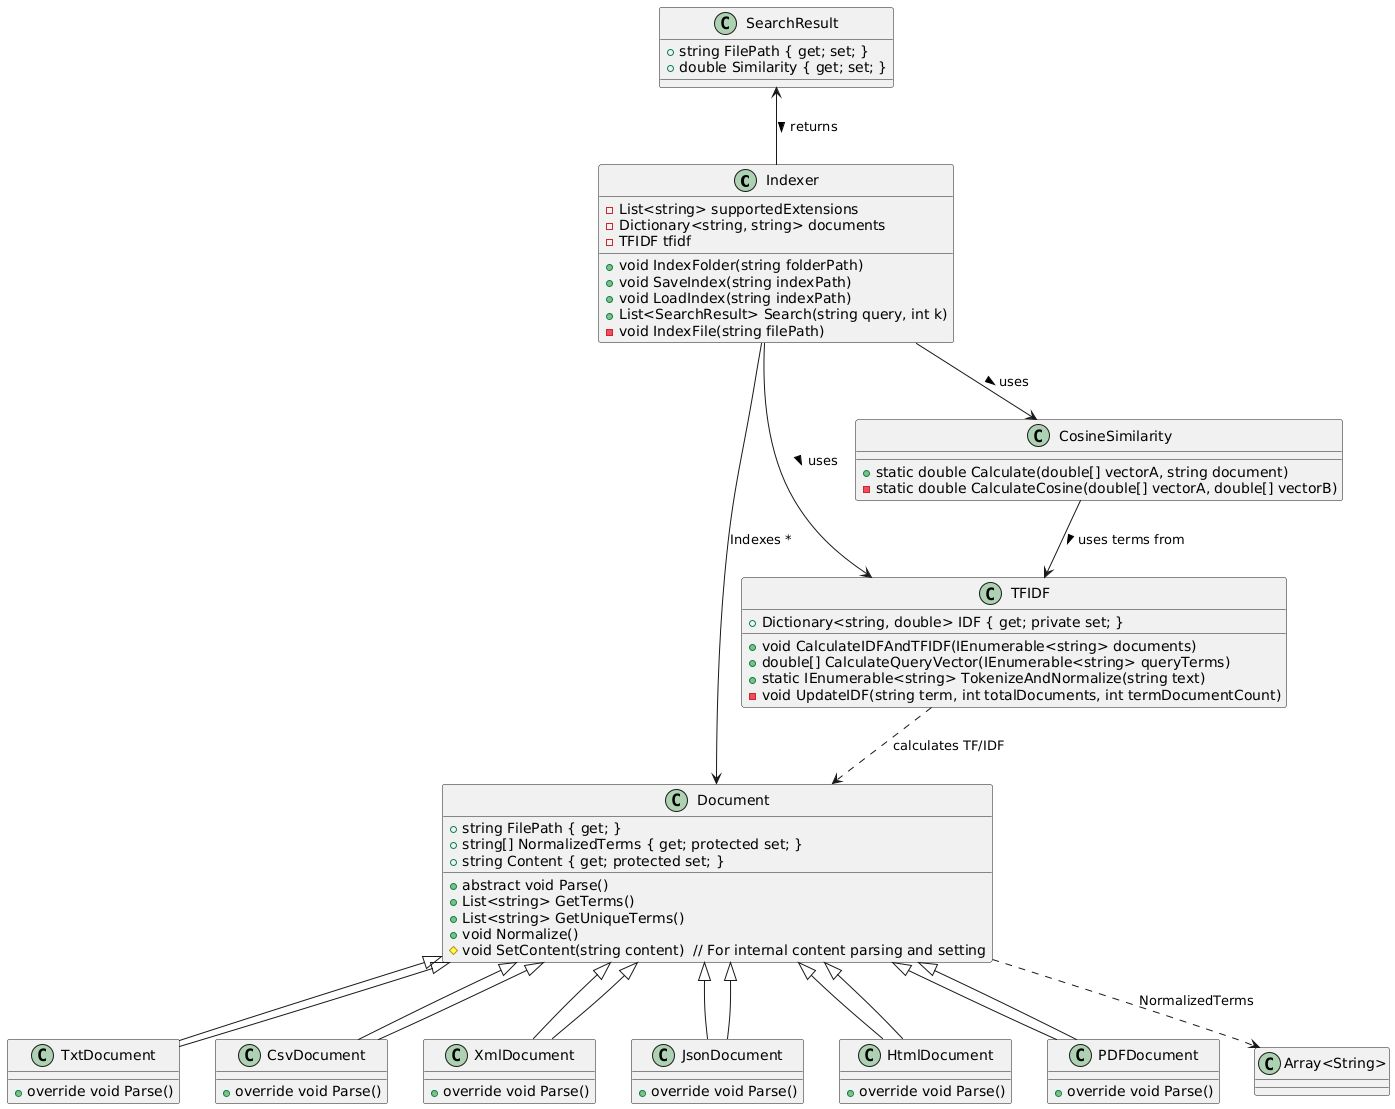
\includegraphics[width=0.5\textwidth]{Image_OriginalClassDiagram.jpeg}
    \caption{Image explaining the Class Diagram we developed at the beginning.}
    \label{fig:OriginalClassDiagram}
\end{figure}
This diagram managed to encompass the overall design we ended up using throughout the development of this code. Yet, various changes ended up being made to the design in the midst of the development process. The class diagram that ended up encompassing the overall flow of the backend of the program is. 
\begin{figure}[H]
    \centering
    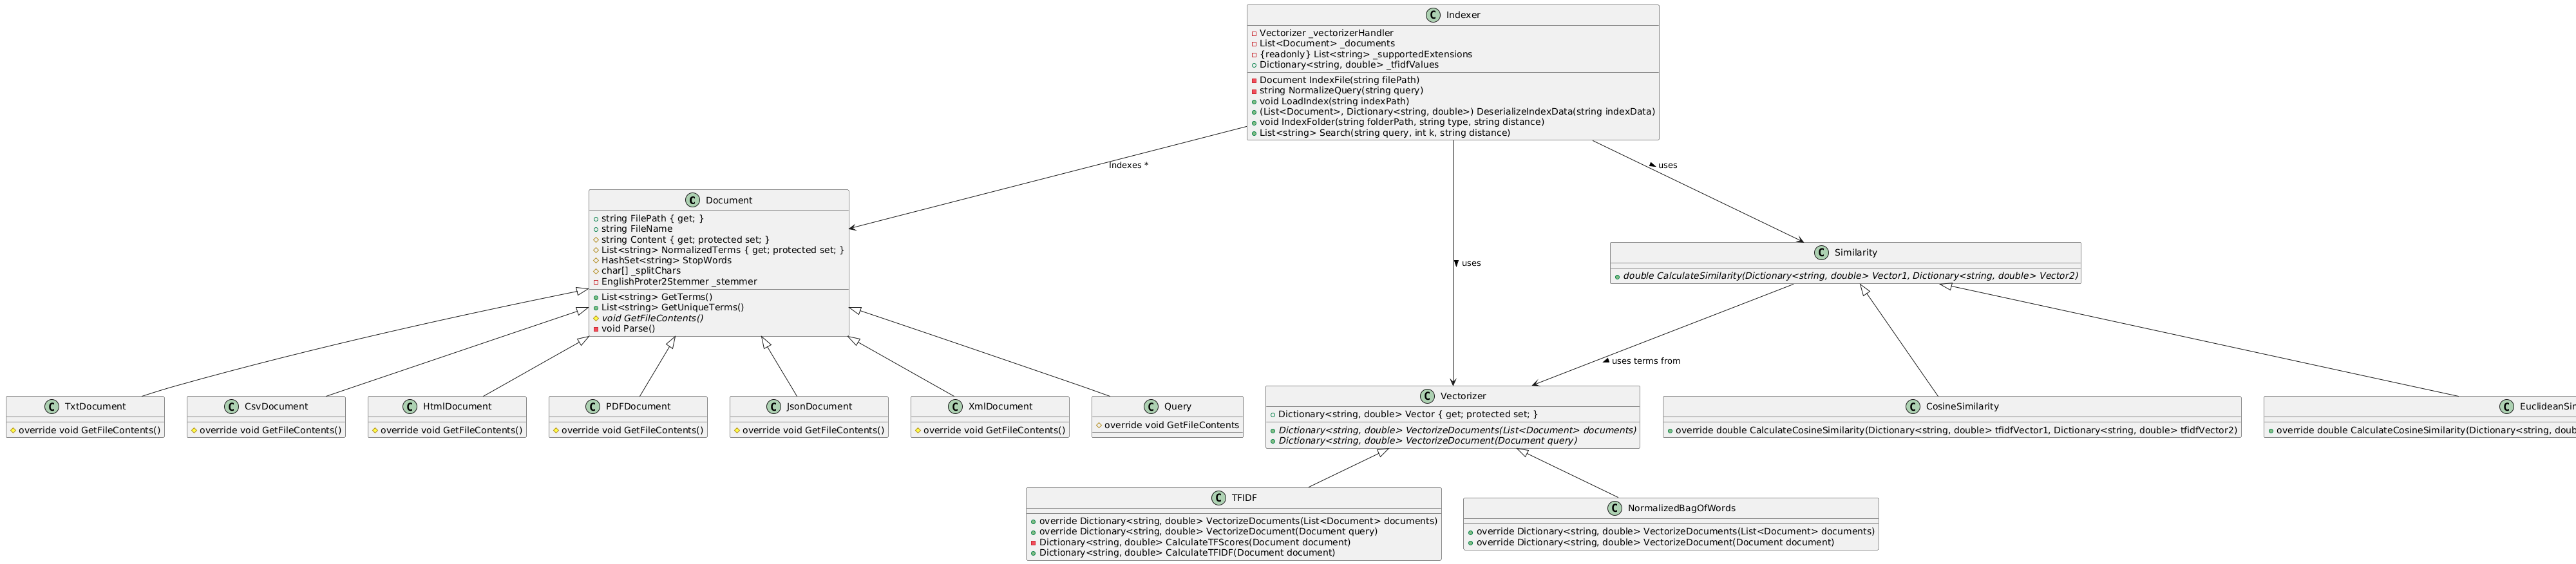
\includegraphics[width=\textwidth]{Image_UpdatedClassDiagram.png}
    \caption{Image explaining the Updated Class Diagram we developed once the backend was complete. The image is cropped in the right side due to the size.}
    \label{fig:UpdatedClassDiagram}
\end{figure}
This diagram contains the end design of the program for the development of the code. It explains the various different classes and their relationships in the code without the need of accessing the program.
\begin{figure}[H]
    \centering
    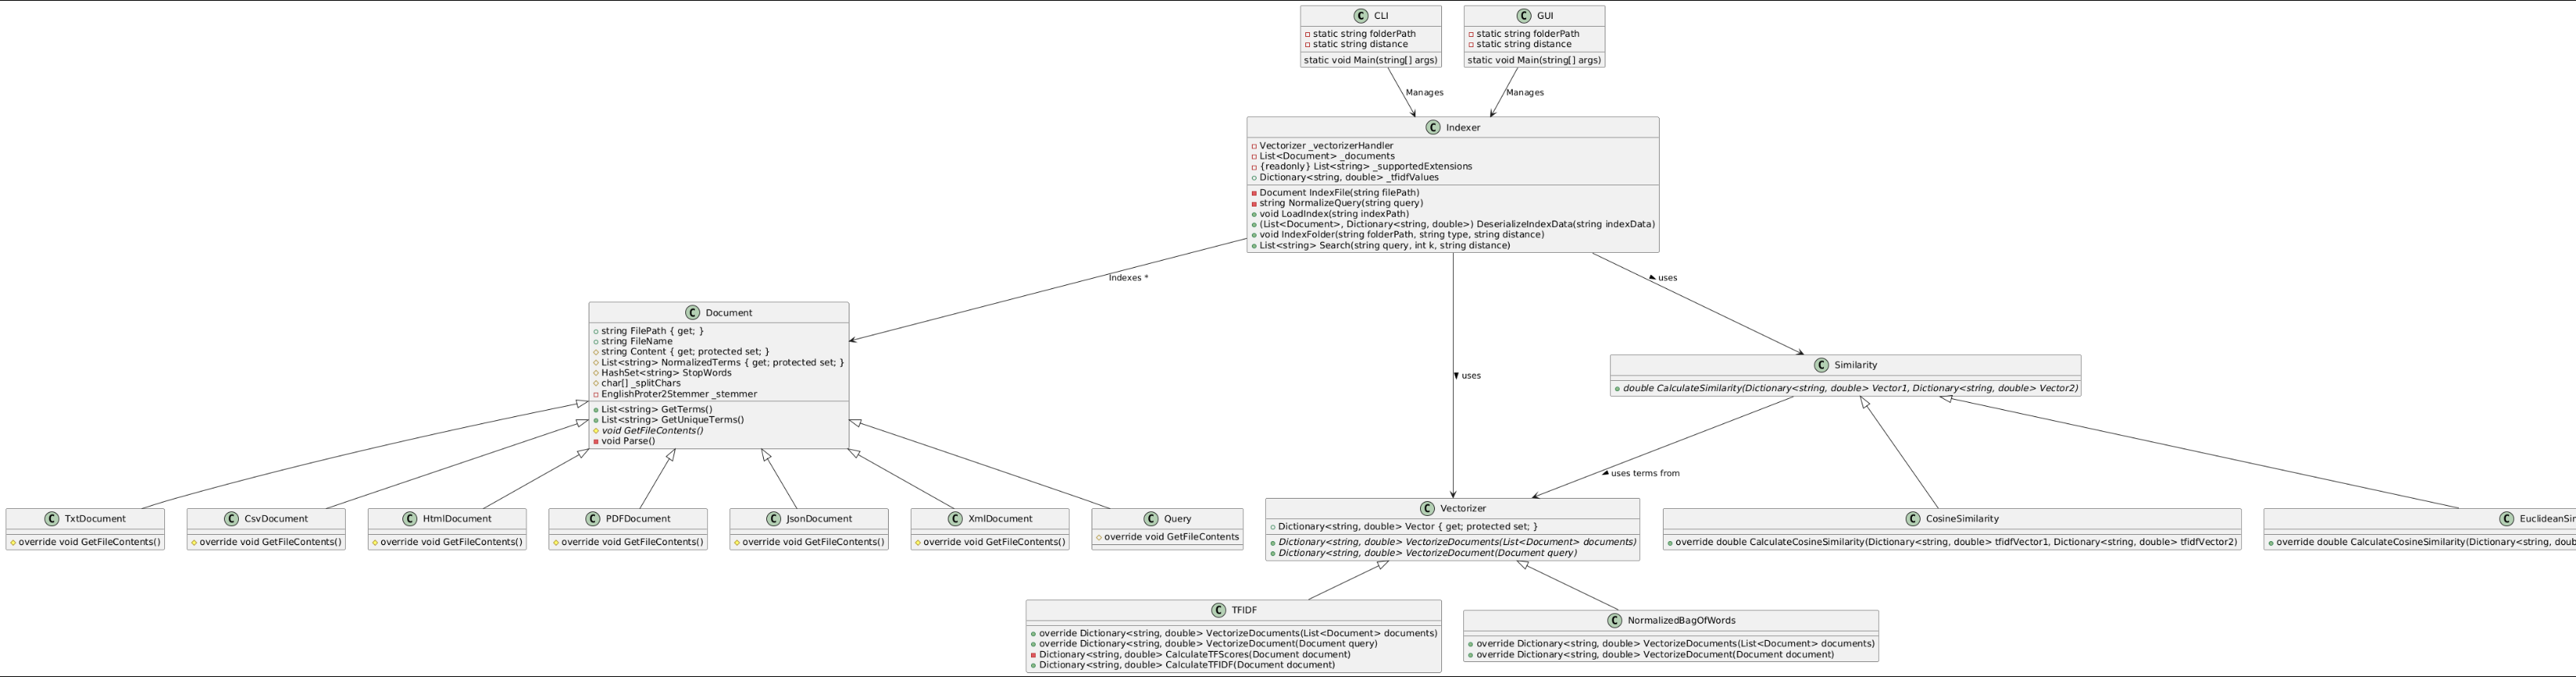
\includegraphics[width=\textwidth]{Image_CliGuiDiagram.png}
    \caption{Image explaining the Class Diagram we developed at the beginning.}
    \label{fig:FinalClassDiagram}
\end{figure}

The final diagram with the end results containing the CLI and the GUI as a class are demonstrated in figure \ref*{fig:FinalClassDiagram}, both use the same format since the handling of these programs was accomodated to the same classes, with no changes on the classes but changes on the interpretations of the user's inputs.

\section{Graphical User Interface (GUI)}
The Graphical User Interface (GUI) for our project was developed using Blazor, a modern web framework that allows for the creation of interactive web applications using C sharp. Blazor enables developers to build client-side web applications with a component-based architecture, which promotes reusability and maintainability of code.

The GUI consists of several components that facilitate user interaction with the indexer/search engine. Key features of the GUI include:

\begin{itemize}
    \item \textbf{Dynamic Routing:} The application uses a router to manage navigation between different pages, such as the home page and the about page. This allows users to seamlessly navigate through the application without full page reloads.
    \item \textbf{Data Binding:} The GUI leverages data binding to connect the user interface with the underlying data model. This ensures that any changes in the data are automatically reflected in the UI, providing a responsive user experience.
    \item \textbf{Event Handling:} User actions, such as button clicks and selections from dropdown menus, are handled through event handlers. This allows the application to respond to user input in real-time, such as executing a search query when the user clicks the search button.
    \item \textbf{Styling and Layout:} The application uses CSS for styling, ensuring a visually appealing and user-friendly interface. The layout is designed to be responsive, adapting to different screen sizes and devices.
    \item \textbf{Integration with Backend Logic:} The GUI communicates with the backend logic of the indexer/search engine, allowing users to perform searches and view results dynamically. This integration is achieved through dependency injection, where services like the `Indexer` are registered and utilized within the components.
\end{itemize}
\subsection{How It Works}
The GUI operates as follows:
\begin{enumerate}
    \item \textbf{User Input:} Users can enter their search queries in a designated textbox. They can also select the vectorization method and distance metric from dropdown menus.
    \item \textbf{Executing a Search:} After entering a query and selecting the desired options, users click the "Search" button. This triggers the search functionality, which processes the query and retrieves the top \( k \) documents based on the specified criteria.
    \item \textbf{Displaying Results:} The search results are displayed in a list format. Users can click on any document title to view its full content. If no results are found, an appropriate message is shown.
\end{enumerate}

The GUI fulfills the following requirements:
\begin{itemize}
    \item \textbf{Query Input:} Users can enter their search queries in a textbox, allowing for easy input of search terms.
    \item \textbf{Search Functionality:} Upon clicking the search button, the application processes the query and retrieves the top \( k \) documents ordered from the most similar to the least similar based on the selected vectorization method and distance metric.
    \item \textbf{Document Access:} Users can click on the document titles in the search results to read the full content of the documents, enhancing the usability of the application.
\end{itemize}

\subsection{About Page}
The About page provides users with an overview of the project, its purpose, and the developers involved. It serves as an informative section that outlines the goals and functionalities of the indexer/search engine. 

Key points included in the About page are:
\begin{itemize}
    \item \textbf{Project Overview:} A brief description of the project, highlighting its role in the curriculum for the Object-Oriented Programming course at Texas Tech University.
    \item \textbf{Functionality:} An explanation of the search engine's capabilities, including recursive folder indexing and the use of algorithms like TF-IDF and Cosine Similarity for document retrieval.
    \item \textbf{User Interfaces:} Information about the two main interaction interfaces: the Command Line Interface (CLI) and the Graphical User Interface (GUI), emphasizing adherence to Object-Oriented Programming principles.
    \item \textbf{Importance of Indexing:} A discussion on the significance of indexing and searching through large collections of documents, drawing parallels to larger search engines.
    \item \textbf{Developers:} A section dedicated to the developers, providing their names and academic status.
\end{itemize}

This page not only informs users about the project but also enhances the overall user experience by providing context and background information.

Overall, the Blazor-based GUI enhances the usability of the indexer/search engine, making it accessible and efficient for users to search through various document types.

\section{Command Line Interface (CLI)}
This section will explain how each command may be inputted into the command line of the program. Following are all command variants that are valid in our project.
\begin{figure}[H]
\begin{itemize}
    \item[$>$] \texttt{index -f $<folderPath>$ -t tfidf -dis cosine}: this command uses the standard method for both the indexer and the search engine, the \textbf{TF-IDF} for indexing and the \textbf{Cosine Similarity} for searching values. 
    \item[$>$] \texttt{index -f $<folderPath>$ -t tfidf -dis euclidean}: this command uses the \textbf{TF-IDF} algorithm for indexing the files and the \textbf{Euclidean Similarity} algorithm for searching values. 
    \item[$>$] \texttt{index -f $<folderPath>$ -t vectorizer -dis euclidean}: this command uses the \textbf{Normalized Bag of Words} algorithm for indexing the files and the \textbf{Cosine Similarity} algorithm for searching values. 
    \item[$>$] \texttt{index -f $<folderPath>$ -t vectorizer -dis cosine}: this command uses the \textbf{Normalized Bag of Words} algorithm for indexing the files and the \textbf{Euclidean Similarity} algorithm for searching values. 
    \item[$>$] \texttt{load -p $<indexPath>$}: uses the path to the "\texttt{.Json}" document that holds the information of an indexed folder.  
    \item[$>$] \texttt{search -q $<query>$ -k $<numberResults>$}: gets the query from the user and the number of results it should return form $<numberResults>$. 
\end{itemize}
\label{fig:Commands}
\end{figure}

The item list mentioned before contains all valid formats of command. All values in between characters '$<$' and '$>$' represent variables in the command which may change depending on what the user wants.

\section{Code Overview}
For this section of the documentation we will be focusing on the back-end of the code. Explaining the overall code structure and how each part correlates to eachother. Let's begin our conversation with the document handling and natural language processing section of the code.
\subsection{Document Hierarchy}
The document hierarchy is the way we ended up organizing how each file is handled. It is composed of a parent class, \textbf{Document} which is in charge of the overall construction of each instance, except for the \textbf{Special Child} / Query, and the contents parsing. 

This class does this by allowing containing the abstract method \texttt{GetFileContents} which each child has a unique method of performing. After, extracting the files contents it finally manages to parse the contents by removing all \textbf{stop words}, \textbf{split chars}, and \textbf{stemming}each word to extract the very essence of the contents of each file\footnote{This algorithm uses the Porter2Stemmer algorithm from: \url{https://www.nuget.org/packages/Porter2Stemmer}}. With the followingmethod:
\begin{figure}[H]
    \begin{lstlisting}[language=C]
    public void Parse(){    
        string[] words = Content.ToLower().Split(_splitChars,
                StringSplitOptions.RemoveEmptyEntries);
        foreach (var term in words) 
        {
            if (!StopWords.Contains(term))
            {
                var stemmedWord = _stemmer.Stem(term);
                NormalizedTerms.Add(stemmedWord.Value);
            }
        }
    }
    \end{lstlisting}
    \caption{Parsing Method. Found in Document.cs.}
    \label{fig:ParseMethod}
\end{figure}
\subsubsection{The Common Children Classes}
The following children classes are named the common children since they all use the same constructor, defined in the base class, but all override the \texttt{GetFileContents} method to fit their respective file to handle. The constructor method they use is the following.
\begin{figure}[H]
    \begin{lstlisting}[language=C]
    public Document() 
    {
        NormalizedTerms = new List<string>();
    }
    public Document(string filePath) : this()
    {   
        FilePath = filePath;
        GetFileContents();
        Parse();
    }
    \end{lstlisting}
    \caption{Constructor Functions. Found in Document.cs.}
    \label{fig:Constructor}
\end{figure}
Each class in the itemized list that follows has this exact same behavior when an instance of itself gets performed. 
\begin{itemize}
    \item[1.] \texttt{CsvDocument Class} 
    \item[2.] \texttt{HtmlDocument Class}
    \item[3.] \texttt{JsonDocument Class}
    \item[4.] \texttt{PDFDocument Class}
    \item[5.] \texttt{TxtDocument Class}
    \item[6.] \texttt{XmlDocument Class}
\end{itemize}
They compose all the files that the code should be able to handle, based on project prerequisites.
\subsubsection{The Special Child}
The \textbf{Special Child} is the QueryDocument Class, which is an abstraction we implemented on the user query to maintain similar modularization throughout 
our code it allowed the query to be treated as a document. It was the only "concrete" class of the Document Hierarchy that never overrided the \texttt{GetFileContents}
method since it never needed to do so. Since, it initialized itself using the following constructor method.
\begin{figure}[H]
    \begin{lstlisting}[language=C]
    public Query(string query) : base()
    {
        if (string.IsNullOrWhiteSpace(query))
        {
            throw new ArgumentException("Query cannot be null or empty.");
        }   
        Content = query; // Assign the query to the content
        Parse();
    }
    \end{lstlisting}
    \caption{Constructor Functions. Found in Document.cs.}
    \label{fig:Constructor2}
\end{figure}
Thus, causing  it and others to use the exact same code for parsing, 
NLP and "document" handling. Lastly, any documents not covered in section 2.1
would appear as null and not handled on other sections.

\subsection{Similarity Hierarchy}
The similarity section of the code is in charge of defining the two different methods of searching the code was expected to have. It contains a single abstract method named \texttt{CalculateSimilarity} that defines that its children should have a way of calculating how similar two vectors are, and based on each child class it performs a different method.
\subsubsection{Cosine Similarity Class}
The \texttt{CosineSimilarity} class is the algorithm we were expected to create for the development of this project. Using vectors it calculates how similar the direction of two vectors is, with the following math formula.

\begin{center}
    \[
        \textbf{Similarity}(A, B) = cos(\theta) = \frac{\mathbf{A} \cdot \mathbf{B}}{\|\mathbf{A}\| \cdot \|\mathbf{B}\|}
    \]
\end{center}

\indent In essence this class override the \texttt{CalculateSimilarity} method to use the similarity mathematical equation. This algorithm, for calculating how similar two vectors are, is very efficient since it works with the direction of the vector so it isn't heavily influenced by disparity in sizes. So, it is pretty good when handling a small query size. To further understand the reuslts of similarities lets look at the following picture.

Yet, it is very computationally intensive for handling big query sizes (\textit{Document Contents as a Query}). That is why we decided on using another algorithm for our implementation of the search engine that would give it more power when handling big query sizes. 

\subsubsection{Euclidean Similarity Class}
The algorithm that would eventually give it this edge in computation is the \texttt{EuclideanSimilarity} class. Which overrides it with a method that allows it to give it this edge. This method is in charge of calculating the difference between documents and returning the inverse output of it. Using this:

\begin{center}
    \[
    \textbf{Similarity}(A, B) = \frac{1}{1 + \sqrt{\sum_{i=1}^{n} (A_i - B_i)^2}}
    \]
\end{center}

\indent Where, the bigger the difference between vectors the closer the less similar the contents of each vector are to eachother. This method is heavily influenced by the disparity in sizes between vectors $A$ and $B$. Thus, it gives us more efficiency with big query sizes, but lacks precision when small query's are utilized. To, further understand the differences between both lets look at images of what each is calculating.

\subsubsection{Differences between the Children}
\begin{figure}[H]
    \centering
    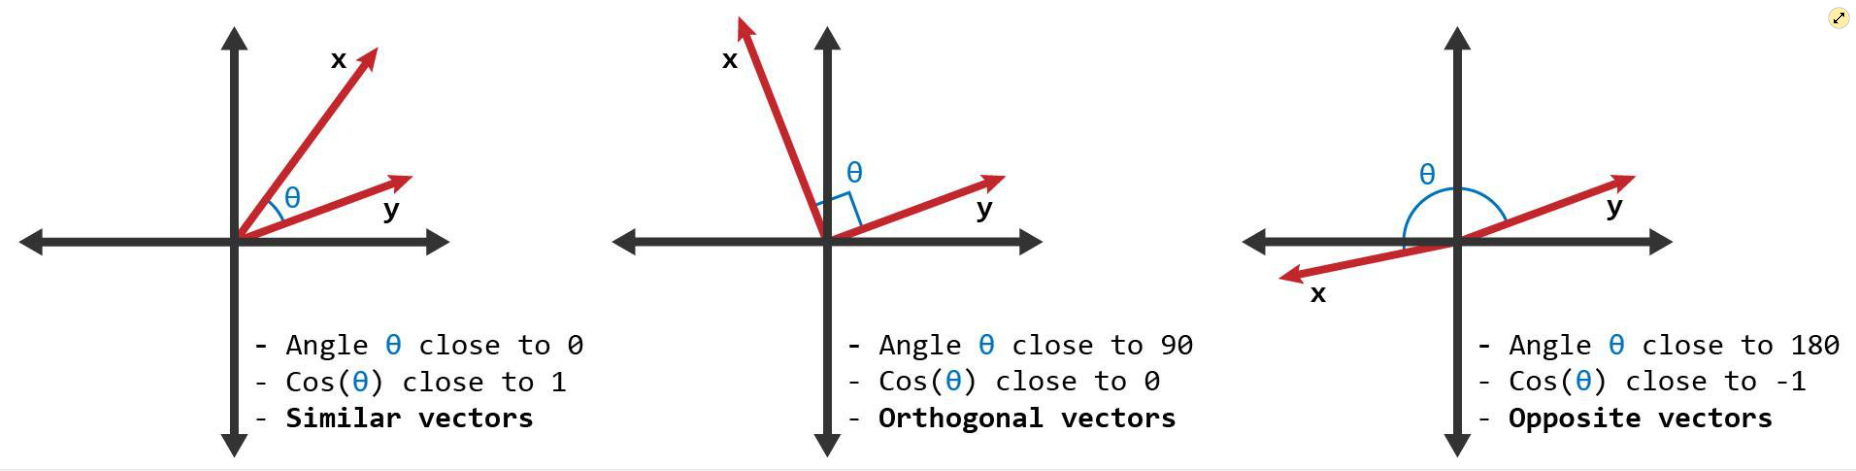
\includegraphics[width=\textwidth]{Image_CosineSimilarity.png}
    \caption{Image for Representing Cosine Similarity. Retrieved from: \url{https://www.learndatasci.com/glossary/cosine-similarity/}}
    \label{fig:CosineSimilarity}
\end{figure}
\begin{figure}[H]
    \centering
    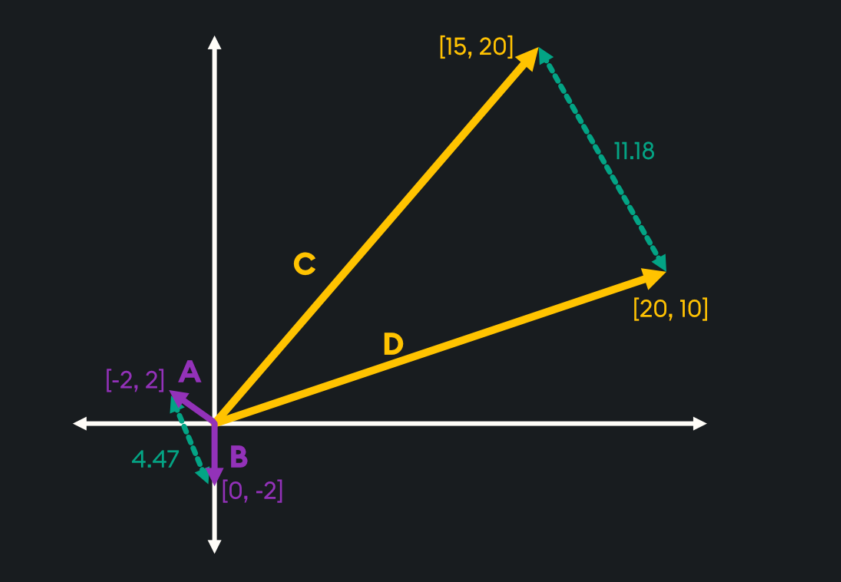
\includegraphics[width=0.8\textwidth]{Image_EuclideanSimilarity.png}
    \caption{Image for Representing Euclidean Similarity. Retrieved from: \url{https://kdb.ai/learning-hub/articles/methods-of-similarity/}}
    \label{fig:EuclideanSimilarity}
\end{figure}
As we can visualize from figure~\ref*{fig:CosineSimilarity} we can understand that the Cosine Similarity looks at the 'similarity' of vectors as directions. Meanwhile in figure~\ref*{fig:EuclideanSimilarity} we understand that Euclidean Similarity looks at it out of how similar each vector is in terms of \textit{magnitude}.
\newline
\indent As a recommendation for users when utilizing the code we developed, I recommend that when looking up queries of \textbf{small sizes} they utilize the Cosine Similarity. Sizes are relative dependent on the average size of the documents in the folder to be indexed.

\subsection{Vectorizer Hierarchy}
The Vectorizer Hierarchy is the class of families in charge of the overall indexing of the folders, it is in charge of creating the abstractions of how the files are interpret in memory. It's named \textbf{vectorizer} due to its ability of vectorizing what is input to it. For the development of this project we decided to create our own indexing algorithm. The first algorithm we used is the \textbf{TF-IDF} algorithm.
\subsubsection{Term Frequency - Inverse Document Frequency (TF-IDF) Algorithm}
The TFIDF child class is in charge of vectorizing each document using the three formulas. The \textbf{Term Frequency (TF)} manages to get the frequency in which each term appears in a document. 
\begin{figure}[H]
    \[
    \text{TF}(t, d) = \frac{f_{t,d}}{\sum_{t' \in d} f_{t',d}}
    \]
    Where, the variables represent:
    \begin{itemize}
        \item \( f_{t,d} \) is the frequency of the term \( t \) in the document \( d \).
        \item \( \sum_{t' \in d} f_{t',d} \) is the sum of frequencies of all terms in the document \( d \).
    \end{itemize}
    \caption{Formula used for Term Frequency calculation of a single term in a document}
    \label{fig:TermFrequency}
\end{figure}
\begin{figure}[H]
    \[
    \text{IDF}(t, D) = \log\left(\frac{N}{| \{ d \in D : t \in d \} |}\right)
    \]
    Where, the terms represent:
    \begin{itemize}
        \item \( N \) is the total number of documents in the corpus \( D \),
        \item \( | \{ d \in D : t \in d \} | \) is the number of documents in which the term \( t \) appears.
    \end{itemize}
    \caption{Formula used for Calculating the Inverse Document Frequency of a single term}
    \label{fig:InverseDocumentFrequency}
\end{figure}
\begin{figure}[H]
    \[
    \text{TF-IDF}(t, d, D) = \text{TF}(t, d) \times \text{IDF}(t, D)
    \]
    \caption{Formula used for Calculating the TFIDF of a document considering the TF and IDF}
    \label{fig:TFIDF}
\end{figure}
For the development of this code we used \textbf{TF-IDF} algorithm as an interpretation of these formulas in code. Considering that each formula returns a vector that can be handled by the other classes of the code. This is one of the abstractions utilized for the vectorization of the files.
\newline
\indent This algorithm was what was expected of us to develop initially for the creation of the \textbf{Indexer and Search Engine}, one of the initial requirements.
\subsubsection{Custom Algorithm: Normalized BoW} 
This algorithm is the other version of the indexer we had to develop, we used a custom algorithm which mixes concepts of the \textbf{Bag of Words}\footnote{A quick explanation of the Bag of Words model is found in: \url{https://www.ibm.com/topics/bag-of-words}} algorithm for indexing, which is just considering each file as a vector which contains the count of each term in a document. We decided on  Normalizing this vector for lenghts to be reduced and for an easier manipulation. Thus, after indexing the files it is easier to handle them since the individual components of the vector now represent the overall relevance of a term in a file. It uses a similar formula to the one explained in figure \ref*{fig:TermFrequency}. This algorithm is a lot less computationally intensive and still maintains appropiate behavior when being handled by the \textbf{Search Engine}.
\subsection{Indexer Class}
The indexer class is in charge of linking the logic of all class hierarchies and the methods that where passed to us as requirements of this code. To create this we must look back at the figure~\ref{fig:Commands} which represent the available levels of functionality of the code. In this class all the logic that ends up retrieving the output of the program is placed here. It allows for the \textbf{GUI} and the \textbf{CLI} to use nearly identical interpretations. 
\section{Unit Test}
The \textbf{Unit Test} section of the code is in charge of checking that all concrete methods, have the expected behavior. We managed to test all the functionality of the code. Yet, certain tests might be missing out due to our lack of experience in developing tests. Even, though we did manage to be properly generate Unit Test for the Document, Similarity, Vectorizer and Indexer hierarchy. The Unit Testing was done in a straightforward manner, where mock documents and instances of classes where generated. For a further understanding please look at the Folder containing the \texttt{UnitTests} for all classes.
\section{References}
\end{document}